\section{Распрацоўка электроннай бібліятэкі}

\subsection{Распрацоўка зыходнага кода}

Для напісання вэб-сайта электроннай бібліятэкі быў абраны фрэймворк Flask,
напісаны на мове праграмавання Python.

Дадзены выбар абумоўлены наступнымі прычынамі:
\begin{enumerate}
    \item веданне распрацоўшчыкам мовы праграмавання Python;
    \item распаўсюджанасць мовы праграмавання Python;
    \item прастата напісання вэб-сайтаў на Flask;
    \item багатыя магчымасці ў пабочных бібліятэках Python;
\end{enumerate}

Flask --- фрэймворк для стварэння вэб-праграм на мове праграмавання Python, які выкарыстоўвае набор інструментаў Werkzeug, а таксама шабланізатар Jinja2. Адносіцца да катэгорыі так званых мікрафрэймворкаў --- мінімалістычны каркас вэб-праграм, якія прадастаўляюць толькі базавыя магчымасці.

Flask забяспечвае наступныя функцыі:
\begin{enumerate}
    \item маршрутызацыя;
    \item статычныя файлы;
    \item jinja2 шаблоны;
    \item доступ да параметраў запыту;
    \item перанакіраванне;
    \item уласныя памылкі;
    \item логі;
\end{enumerate}

У лістынгу \ref{lst: main.py} прадстаўлены зыходны код, які забяспечваю логіку вэб-сайта электроннай
бібліятэкі.

\lstinputlisting[caption={Зыходны код логікі вэб-сайта},%
                            label={lst: main.py},%
                            language=Python]{main.py}

Запіс \textit{@app.route("/", methods =['GET', 'POST'])} з'яўляецца дэкаратам, які ўказвае
адрас старонкі, пры пераходзе на якую выклікаецца функцыя, а таксама метады, якія могуць
быць апрацованыя гэтай функцыяй.

Заўважым, што функцыі вяртаюць карыстальнікам не статычную html-старонку,
але апрацаваны шаблон, у які былі падстаўлены перададзеныя пераменныя
(напрыклад, запіс \textit{return render\_template('catalog.html ', books\_info=books\_info)}).
Гэта дазваляе ствараць дынамічныя вэб-старонкі, кантэкст каторай будзе брацца са сховішча
даных у залежнасці ад апісанай логікі.

Jinja --- гэта шабланізатар для мовы праграмавання Python. Ён падобны да шабланізатару Django, але падае Python-падобныя выразы, забяспечваючы выкананне шаблонаў ў пясочніцы. Гэта тэкставы шабланізатар, таму ён можа быць выкарыстаны для стварэння любога віду разметкі, а таксама зыходнага кода. Ліцэнзаваны пад BSD ліцэнзіяй.

Шабланізатар Jinja дазваляе настрайваць тэгі, фільтры, тэсты і глабальныя пераменныя. Таксама, у адрозненні ад шабланізатара Django, Jinja дазваляе канструктару шаблонаў выклікаць функцыі з аргументамі на аб'ектах.

У лістынгу \ref{lst: jinja2 sample} прадстаўлена частка jinja2 шаблона, у якім
падстаўляецца html-код на кнігі, інфармацыя пра якія была атрыманая з базы даных.


\lstinputlisting[caption={Прыклад jinja2 шаблона},%
                            label={lst: jinja2 sample},%
                            language=html]{sample.jinja2}

У лістынгу \ref{lst: jinja2 sample} html-элемент, які апісвае адну кнігу,
знаходзіцца ўнутры 2 цыклаў \textit{for}, якія забяспечваюць дубліраванне
дадзенага html-элемента неабходную колькасць разоў і размяшчэнне яго
ў колькасці 3 кніг на 1 радок.

\subsection{Распрацоўка вэб-дызайна}

Для напісання вэб-дызайна электроннай бібліятэкі, было вырашана скарыстацца шаблонамі Bootstrap с пэўнымі
змяненнямі пад патрэбныя задачы (напрыклад, дынамічны кантэнт).

Bootstrap --- свабодны набор інструментаў для стварэння сайтаў і вэб-праграм. Уключае ў сябе HTML і CSS-шаблоны афармлення для тыпаграфікі, вэб-формаў, кнопак, блокаў навігацыі і іншых кампанентаў вэб-інтэрфейсу, уключаючы JavaScript-пашырэння.

Перавагі фреймворка Bootstrap:
\begin{enumerate}
    \item высокая хуткасць распрацоўкі макетаў старонак сайта. Bootstrap змяшчае велізарны набор гатовых рашэнняў і элементаў;
    \item кросбраўзернасць і адаптыўнасць сайта. Усе элементы фрэймворка адаптыўныя пад усе прылады і карэктна адлюстроўваюцца ва ўсіх сучасных браўзeрах.
    \item лёгкасць ў выкарыстанні. Нават чалавек, які мае базавыя веды аб HTML і CSS, можа свабодна ствараць вэб-старонкі з выкарыстаннем фрэймворка;
    \item прастата ў навучанні. У Bootstrap вельмі добрая дакументацыя з вялікай колькасцю прыкладаў гатовага кода.
\end{enumerate}

Пры вёрстцы адаптыўнага класічнага макета: шапка сайта (header), асноўная частка (content), бакавыя калонка (sidebar) і ніз сайта (footer), для карэктнага адлюстравання нам трэба разлічыць шырыню ў працэнтах кожнага элемента і прысвоіць значэнне. Калі з шапкай і футерам усё зразумела, у большасці выпадкаў шырыня будзе 100\%, то для асноўнай часткі кантэнту і бакавой калонкі можа быць 70/30 або 85/25, але пры памяншэнні экрана нас гэта не задаволіць, трэба будзе рабіць па 100\%.

Для такіх мэтаў і патрэбна сетка Bootstrap. Проста задаюцца класы для блокаў, якія паказваюць, якую шырыню павінен займаць элемент і як ён будзе адлюстроўвацца на розных прыладах. Сетка функцыянуе як табліца, у якой ёсць свае радкі і слупкі, максімальную колькасць слупкоў 12.
Акрамя сеткі існуе вялікая колькасць разнастайных кампанентаў: навігацыйныя меню, формы, табліцы, мадальныя вокны, ўкладкі, абвесткі, усплывальныя падказкі і г.д..
Яшчэ вельмі зручна, што платформа Bootstrap дазваляе як загрузіць увесь фрэймворк цалкам, так і толькі тыя кампаненты, якія патрэбныя.

На малюнках \ref{img: sign up sample} і \ref{img: catalog sample} прадстаўлены прыклады дызайну для старонкі
рэгістрацыі і старонкі каталога кніг.

\begin{figure}[h!]
    \centering
    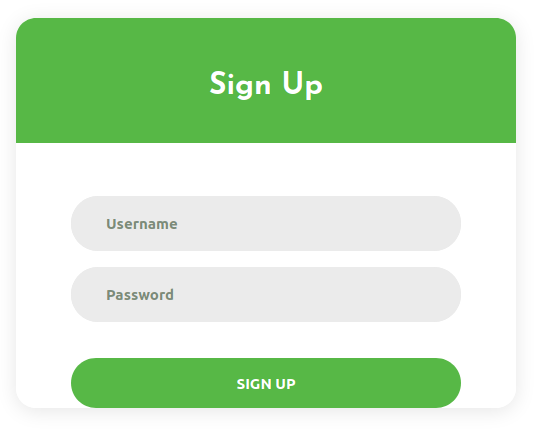
\includegraphics[width=0.7\textwidth]{sign_up}
    \caption{Дызайн старонкі рэгістрацыі}
    \label{img: sign up sample} 
\end{figure}

\begin{figure}[h!]
    \centering
    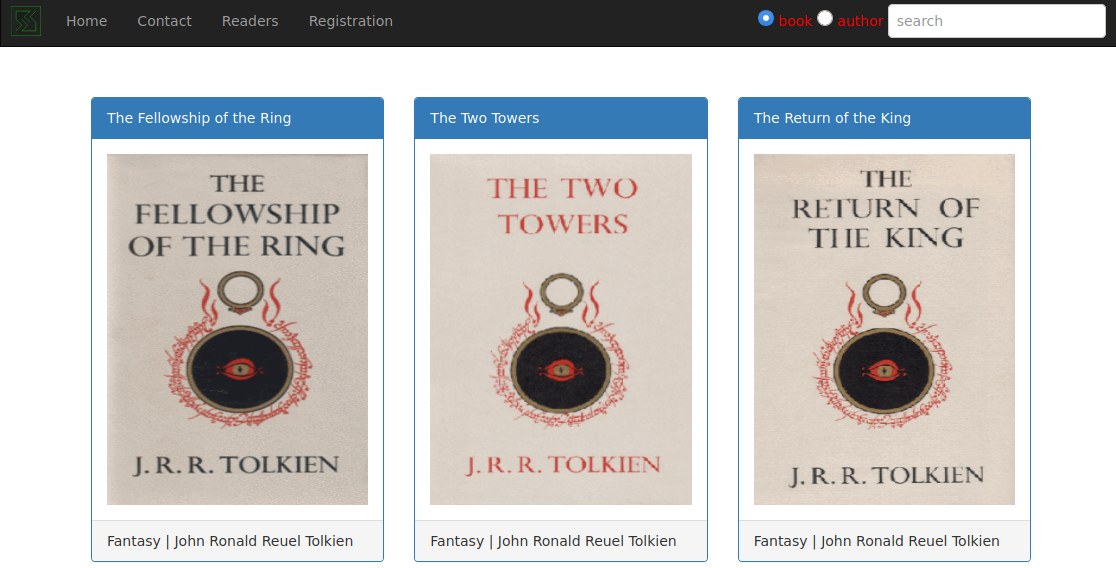
\includegraphics[width=\textwidth]{catalog}
    \caption{Дызайн старонкі каталога кніг}
    \label{img: catalog sample} 
\end{figure}

На старонцы рэгістрацыі былі дабаўленыя дадатковыя функцыі, якія апрацоўваюць памылкі пустых палёў уводу
(username і password) і памылку пры рэгістрацыі чытача з імём, якое ўжо існуе ў базе.

На малюнках \ref{img: sign up error} і \ref{img: sign up error 2} паказаны дызайн вышэй апісаных функцый.

\begin{figure}[h!]
    \centering
    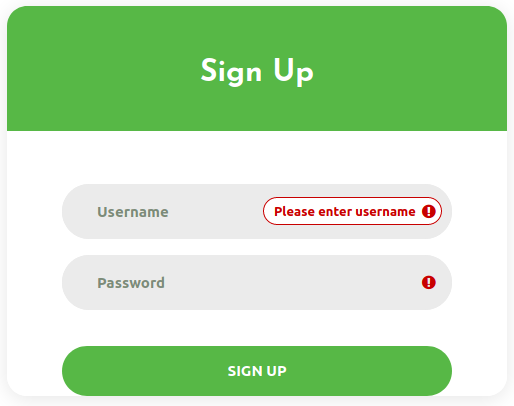
\includegraphics[width=0.7\textwidth]{sign_up_error}
    \caption{Дызайн старонкі рэгістрацыі пры рэгістрацыі з пустым полем ўводу}
    \label{img: sign up error} 
\end{figure}

\begin{figure}[h!]
    \centering
    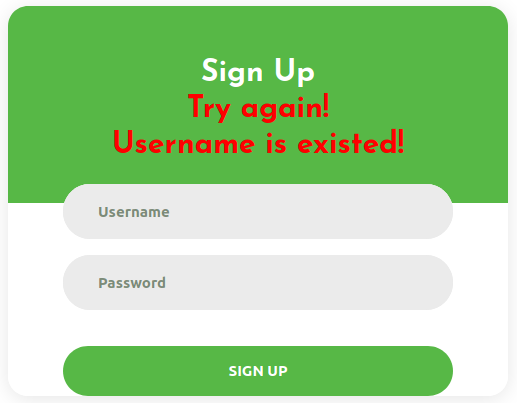
\includegraphics[width=0.7\textwidth]{sign_up_error_2}
    \caption{Дызайн старонкі рэгістрацыі пры рэгістрацыі з існуючым імем}
    \label{img: sign up error 2} 
\end{figure}

\subsection{Дастаўка сервіса}

Для спрашчэння пераходу вэб-сайта на новыя версіі і разгортвання вэб-сайта ў сістэмы было вырашана
разгортваць вэб-сайт унутры Docker кантэйнера. Гэта дазваляе простай заменай старога кантэйнера на новы
змяняць версію вэб-сайта без неабходнасці дадатковых змяненняў сістэмнай канфігурацыі (напрыклад, абнаўлення
версій неабходных пакетаў, бібліятэк)

Docker --- праграмнае забеспячэнне для аўтаматызацыі разгортвання і кіравання праграмамі ў асяроддзях з падтрымкай кантэйнерызацыі. Дазваляе «спакаваць» праграму з усім яго асяроддзем і залежнасцямі ў кантэйнер, які можа быць перанесены на любую Linux-сістэму з падтрымкай cgroups ў ядры, а таксама дае асяроддзе па кіраванні кантэйнерамі.

У лістынгу \ref{lst: Dockerfile} прадстаўлены Dockerfile, пры дапамозе якога будуецца Docker вобраз з
праграмай <<Электронная бібліятэка>> ўнутры.

\lstinputlisting[caption={Dockerfile для будавання Docker вобраза},%
                            label={lst: Dockerfile},%
                            language=bash]{Dockerfile.docker}

Радок \textit{FROM python :3.7-alpine} паказвае, на базе якога Docker вобраза будзе стварацца наш
уласны катэйнер.

Радок \textit{RUN pip3 install mysql-connector-python flask} выконвае ўстаноўку неабходных набор праграм у
Docker вобраз.

Радкі \textit{WORKDIR elibrary} і \textit{COPY elibrary .} указваюць працоўную дырэкторыю Docker вобраза і
капіруюць дырэкторыю праекта (elibrary) у Docker вобраз.

Радок \textit{EXPOSE 5000} рэзервуе порт пры запуску кантэйнера з дадзенага вобразу.

Радок \textit{CMD python3 main.py} вызначае, якая каманда будзе выконвацца пры запуску кантэйнера з дадзенага
Docker вобраза.
